
\section{Desarrollo}

Después de haber realizado el análisis inicial de el alcance del proyecto y las necesidades de los usuarios, se comenzó con el desarrollo del proyecto. Este desarrollo se hizo en tres partes. Primero, el desarrollo de un módulo de monitoreo de las estaciones meteorológicas por medio de drivers,  después un API como intermediaria entre la información almacenada en la base de datos y una interfaz gráfica para el monitoreo eficaz.

\subsection{Del módulo de monitoreo de estaciones}

El módulo de monitoreo de estaciones meteorológicas tiene como objetivo el observar la información obtenida por los diversos drivers de conexión a las estaciones meteorológicas y generar reportes conforme sea necesario, la lógica de reporte es tal como se muestra en la figura \ref{fig:logica_de_reporte}.

%! Agregar acciones al diagrama
%! Cambiar por diagrama de secuencia
% Agregar un fin después de generar la alerta
% debe hber un solo inicio y final

\begin{figure}[!ht]
	\centering
	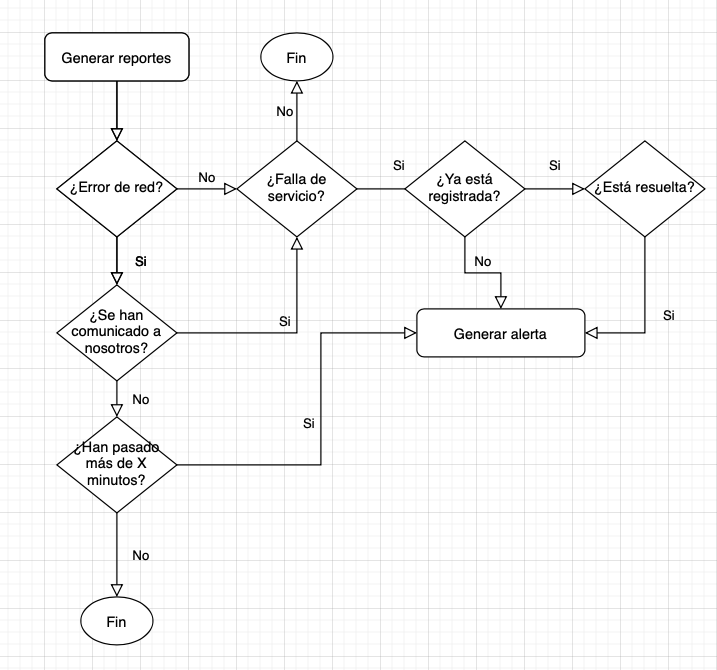
\includegraphics[width=1\linewidth]{images/diagrams/report_logic.png}
	\caption{Lógica de reporte del estado de las estaciones meteorológicas}
	\label{fig:logica_de_reporte}
\end{figure}


\subsection{Del API para el acceso a la información}

\subsection{De la interfaz gráfica del proyecto}

PAra el desarrollo del proyecto, se utilizó tailwind.

\section{Avances}


\section{Módulo de monitoreo}

\subsection*{Requisitos}

\subsection*{Seguridad}

\subsection*{Método de conexion}
